\section{Artefact Design} \label{sec:artefact-design}

As the study evaluated in this thesis is not published, its design is described in the following sections. This thesis reuses the data collected in the study and re-evaluates it under the research questions established for this thesis, providing the rationale for the choices made along the way. Together with the development of the chatbot systems used in the study, this constitutes the artefact design step (step \rom{5}) of the method for design principle development \parencite{Moeller2020} introduced in Section~\ref{ssec:mdpd}. Section~\ref{ssec:setting-participants} describes the study's setting: problem selection, the experiment procedure, and the participants. Section~\ref{ssec:chatbot-construction} describes the construction of the chatbots used in the study.

\subsection{Setting \& Participants} \label{ssec:setting-participants}

The study was designed as mixed-methods study with a between-subjects comparison. Participants were presented three tasks from a pool of maths problems and were asked to solve them with the help of a chatbot. Participants were split into two groups, that received different chatbots. The chatbot for group (E) provided \ac{CoT} explanations for its outputs, while the chatbot for the control group (B) did not. Quantitative data was collected through the task presentation tool and post-experiment questionnaires. Qualitative data was collected through think-aloud protocols during the task solving. Additional qualitative data was gathered based on unprompted feedback from participants after the experiment concluded.

\subsubsection{Problem Selection} \label{sssec:problem-selection}

Problem selection was guided by two criteria: \enquote{ease of access}, referring to the availability of problems and their correct solutions, and \enquote{complexity}, referring to their level of difficulty. Increasing complexity further would have narrowed the pool of participants able to attempt the tasks unaided, reinforcing the trade-off against ease of access. The problems needed to be complex enough to warrant chatbot assistance and to produce meaningful think-aloud protocols, while remaining solvable by a wide range of potential participants. Inspired by \textcite{Wang2024b}, the problems were drawn from the \enquote{testmini} split of the MathVista dataset \parencite{MathVista2024}, chosen for its publicly available solutions and suitable complexity: the natural-language problems, often combined with an image, require multiple steps and the combination of linguistic and visual information to solve. The MATH dataset \parencite{Hendrycks2021} was considered as an alternative, but its open-answer format and lack of multimodality made it less suitable.

% TODO: add examples of problems from MathVista and MATH dataset?

The pool was pre-selected based on the researcher's classification into three difficulty tiers (easy, medium, hard). Pre-testing with non-participant volunteers showed \enquote{easy} problems to be too simple to produce meaningful think-aloud protocols, leaving a final pool of nine problems (five \enquote{difficult}, four \enquote{medium}), which were translated into German to reduce the language barrier for participants.

\subsubsection{Experiment Procedure} \label{sssec:experiment-procedure}

Experiments were conducted as one-on-one sessions between each participant and the researcher, lasting approximately 60 minutes and conducted in a quiet room to minimise distractions and improve the quality of the audio recordings for the think-aloud protocols. The procedure followed three phases, inspired by the experiments performed by \textcite{Jussupow2021} and \textcite{Kazemitabaar2024}: an introduction, the task-solving phase, and a post-experiment questionnaire.

During the introduction, participants were welcomed and provided an overview of the procedure, the think-aloud protocol, and the chatbot. To reduce stress felt by participants, a cover story framed the chatbot itself as the artefact under evaluation; this plausibly directed participants' attention onto the chatbot specifically, which may have helped mitigate — though not eliminate — the risk of attributions toward the chatbot going unverbalised. The researcher then demonstrated the chatbot's key features (multi-modal input, explanations for group (E)), before participants completed a practice task \parencite{VanSomeren1994} to familiarise themselves with the procedure of thinking aloud and the chatbot.

In the task-solving phase, participants were given three randomly selected tasks in sequence, assisted at their discretion by the chatbot, a scientific calculator, and pen and paper, while being encouraged to think aloud throughout \parencite{VanSomeren1994}. No time limit was set, but participants could request a new problem if they felt the current one was unsolvable. The researcher was present to observe and take notes, intervening only to provide technical assistance if needed or to encourage participants to think aloud if they were silent for an extended period of time.

The post-experiment questionnaire comprised a demographic questionnaire, the \ac{TAM} questionnaire \parencite{Davis1989}, the \ac{CSE} questionnaire \parencite{Compeau1995}, and the \acs{NASA}-\ac{TLX} questionnaire \parencite{Hart1988}, all administered in German with items translated from their original English versions by the researcher; the questionnaires are included in the Appendix.

The audio recordings of the think-aloud protocols were transcribed using OpenAI Whisper \parencite{Radford2023} and manually corrected by the researcher, then combined with the chatbot's chat logs and the researcher's notes for the subsequent analysis.

\subsubsection{Participants} \label{sssec:participants}

Participants were recruited through convenience sampling from two sources: (1) students recruited through the chair of Enterprise Computing at the TU Dortmund, and (2) colleagues and acquaintances of the researcher. These channels were chosen to reach participants with a background in \ac{STEM}, to ensure a basic level of mathematical proficiency required for the tasks. Participants were split pseudo-randomly into the two groups (E) and (B), by alternately assigning participants to the groups as they were recruited.

In total 20 participants were asked to take part in the study, of which 15 responded to the recruitment message. Thirteen participants were able to schedule an experiment session, with two participants dropping out due to time constraints. The final sample consisted of 12 participants, as one participant was excluded from the analysis, due to unusable think-aloud protocols. The participant selection process is visualised in the flowchart in Figure~\ref{fig:part-flow}.

\begin{figure}[ht]
    \centering
    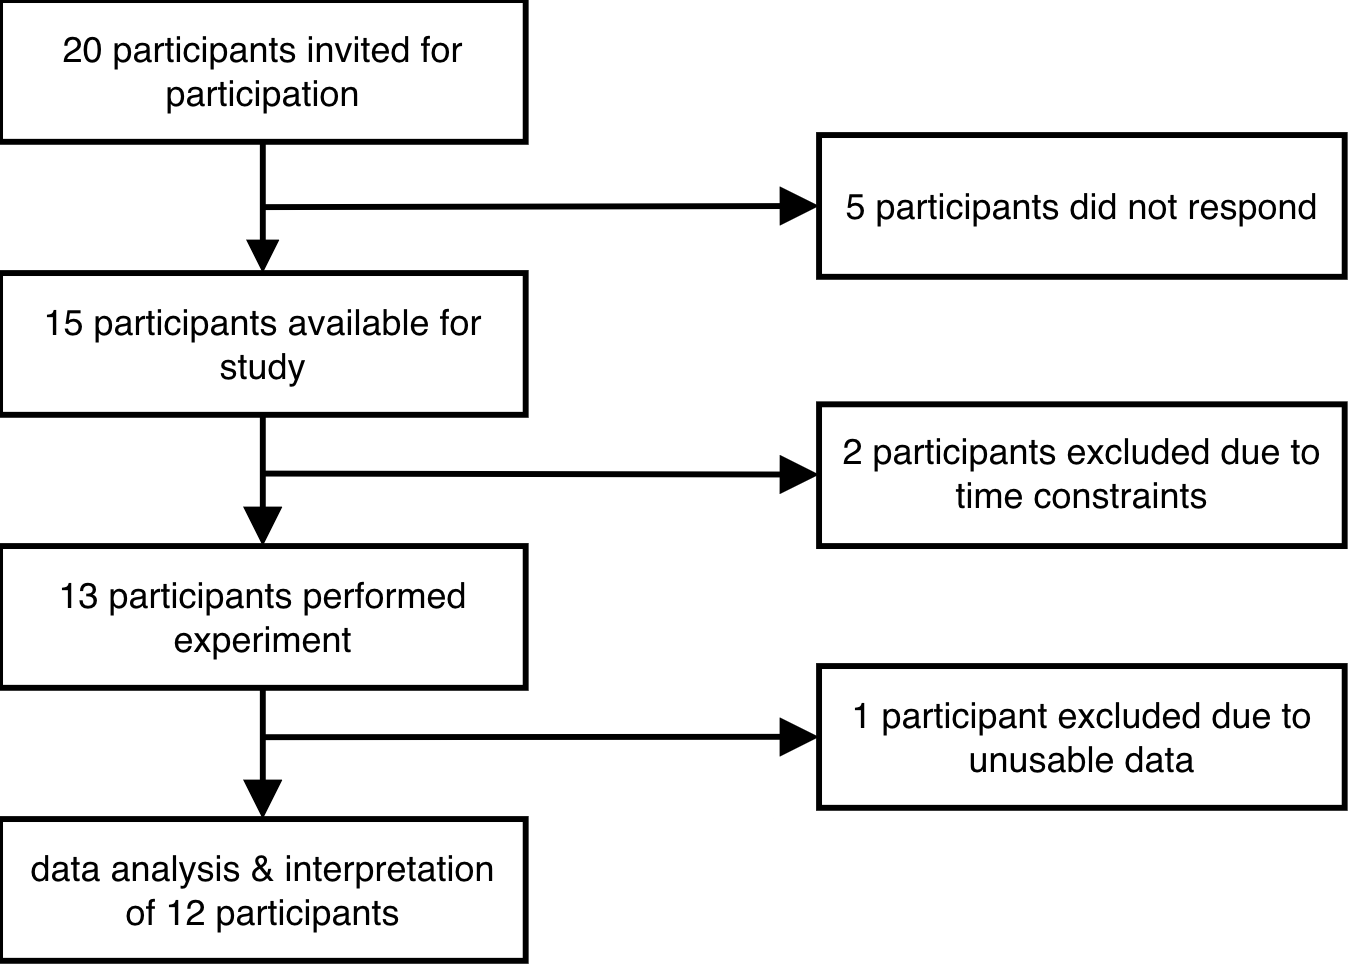
\includegraphics[width=0.6\textwidth]{images/fig-participant_flowchart.png}
    \caption{Participant selection flowchart}
    \label{fig:part-flow}
\end{figure}

The final sample consisted only of male participants, with 7 participants in group (E) and 5 participants in group (B). Additional information about the participants can be found in Tables~\ref{tab:part-age} and \ref{tab:part-edu}.

\begingroup
\tablespacing

\begin{table}[ht]
    \parbox{.45\linewidth}{
        \centering
        \begin{tabular}{c c}
            \toprule
            Age Range & Count \\
            \midrule
            20--29 & 8 \\
            30--39 & 2 \\
            40--49 & 1 \\
            60--69 & 1 \\
            \bottomrule
        \end{tabular}
        \caption{Age distribution of participants}
        \label{tab:part-age}
    }
    \hfill
    \parbox{.45\linewidth}{
        \begin{tabular}{c c}
            \toprule
            Education Level & Count \\
            \midrule
            University Degree & 8 \\
            Vocational Training & 2 \\
            Grammar School & 2 \\
            \bottomrule
        \end{tabular}
        \caption{Educational background of participants}
        \label{tab:part-edu}
    }
\end{table}

\endgroup

Participants were recruited almost exclusively through the personal network of the researcher, with only one participant of the final sample recruited through the university chair. They were not compensated for their participation, but were offered a debriefing after the experiment, in which they were informed about the purpose of the study. Each participant was assigned a unique participant ID, used to link their responses with their questionnaire data and to anonymise audio recordings, transcriptions, and chat logs for the analysis.

\subsection{Chatbot Construction} \label{ssec:chatbot-construction}

Two software components were required for the study: a tool for presenting tasks and recording responses, and the chatbots used by participants for task-solving. As the chatbot was not itself the artefact evaluated by the study, but rather a means to investigate the effects of explanations on users, both components were guided primarily by practical constraints, rather than by an aim to optimise performance or user experience beyond what was necessary for the study:

% ---
% New requirement IDs replace the retired C1-C4 / CR1-CR3 scheme:
%   R1 = C1 (effort) + C2 (cost), merged
%   R2 = C4 (regulation)
%   R3 = CR1 (chatbot must not solve problems outright)
%   C3 (usability) and CR2/CR3 are not carried forward as formal IDs;
%   usability is discussed qualitatively below where relevant.
% ---
\begin{enumerate}[label=(\textbf{R\arabic*}),leftmargin=3em]
    \item The study was carried out by a single researcher within one semester and was self-funded, so tool implementation needed to be efficient and free of monetary cost.
    \item Tools needed to comply with German data protection regulation (GDPR) and additional regulatory burdens for research studies, favouring local or university-hosted data storage.
    \item The chatbot must not solve the problems for participants outright, but only provide assistance in the form of hints and explanations, to ensure participants collaborated actively with the chatbot and produced meaningful think-aloud protocols.
\end{enumerate}

Usability was a partial corollary of these constraints; its influence on specific choices is noted below.

A custom web application (Next.js) was built to present tasks to participants and record their responses, with source code available in a public repository \parencite{Goepfert2025}. Figure~\ref{fig:task-tool} shows the task tool interface.

% TODO: swap this screenshot for one showing a different example task from the pool, so it also serves as an implicit example-task illustration; check whether the caption still needs adjustment afterwards.
\begin{figure}[ht]
    \centering
    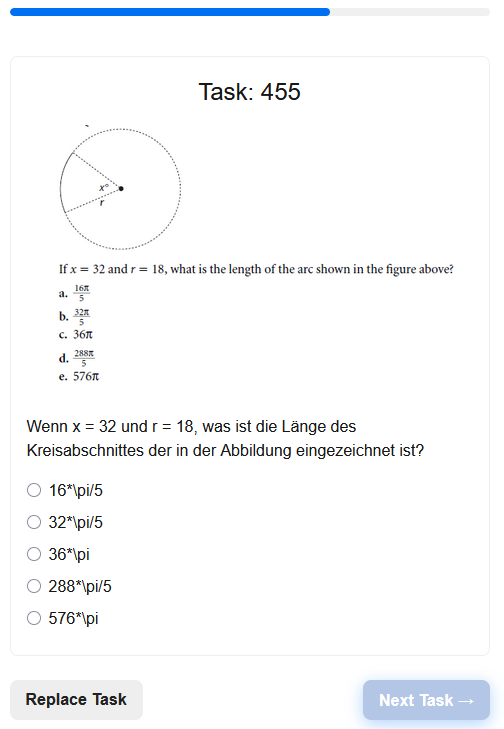
\includegraphics[width=0.5\textwidth]{images/fig-task_viewer.png}
    \caption[Screenshot of the task tool]{Screenshot of the task tool with simple column layout. At the top a progress bar shows the progress for participants. Below that the task is displayed with the task ID, the image, the translated task text and response options. Below the tasks are buttons to replace the current task and progress to the next task, once a response is given.}
    \label{fig:task-tool}
\end{figure}

The chatbot required more deliberate design, as it needed to remain functional and usable for participants while respecting the constraints above. An offline \ac{LLM}, run locally through LM Studio, was selected to power it (\textbf{R1}, \textbf{R2}). Candidate models were identified via Hugging Face, filtering for parameter counts under 30 billion and release dates from 2024 onward; after removing duplicates, three models remained for evaluation: Gemma 3 27B \parencite{GemmaTeam2025}, Mistral Small 3.2 \parencite{Mistral2025}, and Qwen 30B \parencite{Qwen2025}. System prompts were designed to elicit the desired behaviour, identical between the two chatbot variants except for a zero-shot chain-of-thought instruction \parencite{Wei2022, Kojima2022} added for group (E).

% TODO: pending decision whether to keep the Qwen-elimination detail below, or cut it if space runs short.
Each candidate was tested against problems from the pool and evaluated on response quality against \textbf{R3}. Qwen 30B was eliminated, as it frequently solved problems outright rather than only providing hints, violating \textbf{R3}. Gemma 3 and Mistral Small 3.2 performed comparably; Mistral Small 3.2 was ultimately selected, as Gemma's more verbose responses were expected to be less user-friendly for participants and to increase the risk of the chatbot inadvertently solving problems for participants (\textbf{R3}).

\ac{CoT} explanations were chosen as the explanation mechanism for group (E) over the LIME and SHAP methods introduced in Section~\ref{sssec:xai-methods}, primarily on grounds of feasibility: unlike LIME and SHAP, which do not transfer well to generative models and require surrogate-model machinery, \ac{CoT} explanations can be elicited through training or even zero-shot prompting, and so can be implemented with minimal technical overhead \parencite{Wei2022, Kojima2022}.

Adding a \ac{CoT} instruction to only the explanation group's system prompt introduces a dual manipulation: beyond the presence of a visible explanation, \textcite{Wei2022} report that \ac{CoT} prompting can itself improve response quality on complex tasks, so a between-group difference cannot be cleanly attributed to the presence of an explanation alone. Isolating this confound would have required a substantially more complex study design, outside the scope available to a single researcher in one semester (\textbf{R1}); this trade-off was accepted for the study reported here.

Since both chatbot variants were implemented in LM Studio, the interface was identical for both groups, ensuring that the presence of explanations was the only difference between them. Through the system prompt, the chain of thought was wrapped in an HTML-style \texttt{<think>} tag, rendered as a collapsed, click-to-expand element. Figure~\ref{fig:chatbots} shows screenshots of the introductory task demonstration for both chatbots.

% TODO: confirm whether the source screenshots themselves need updating for the (C) -> (B) group-label fix, if the label is visible in the UI.
\begin{figure}[ht]
    \centering
    \begin{subfigure}{0.49\textwidth}
        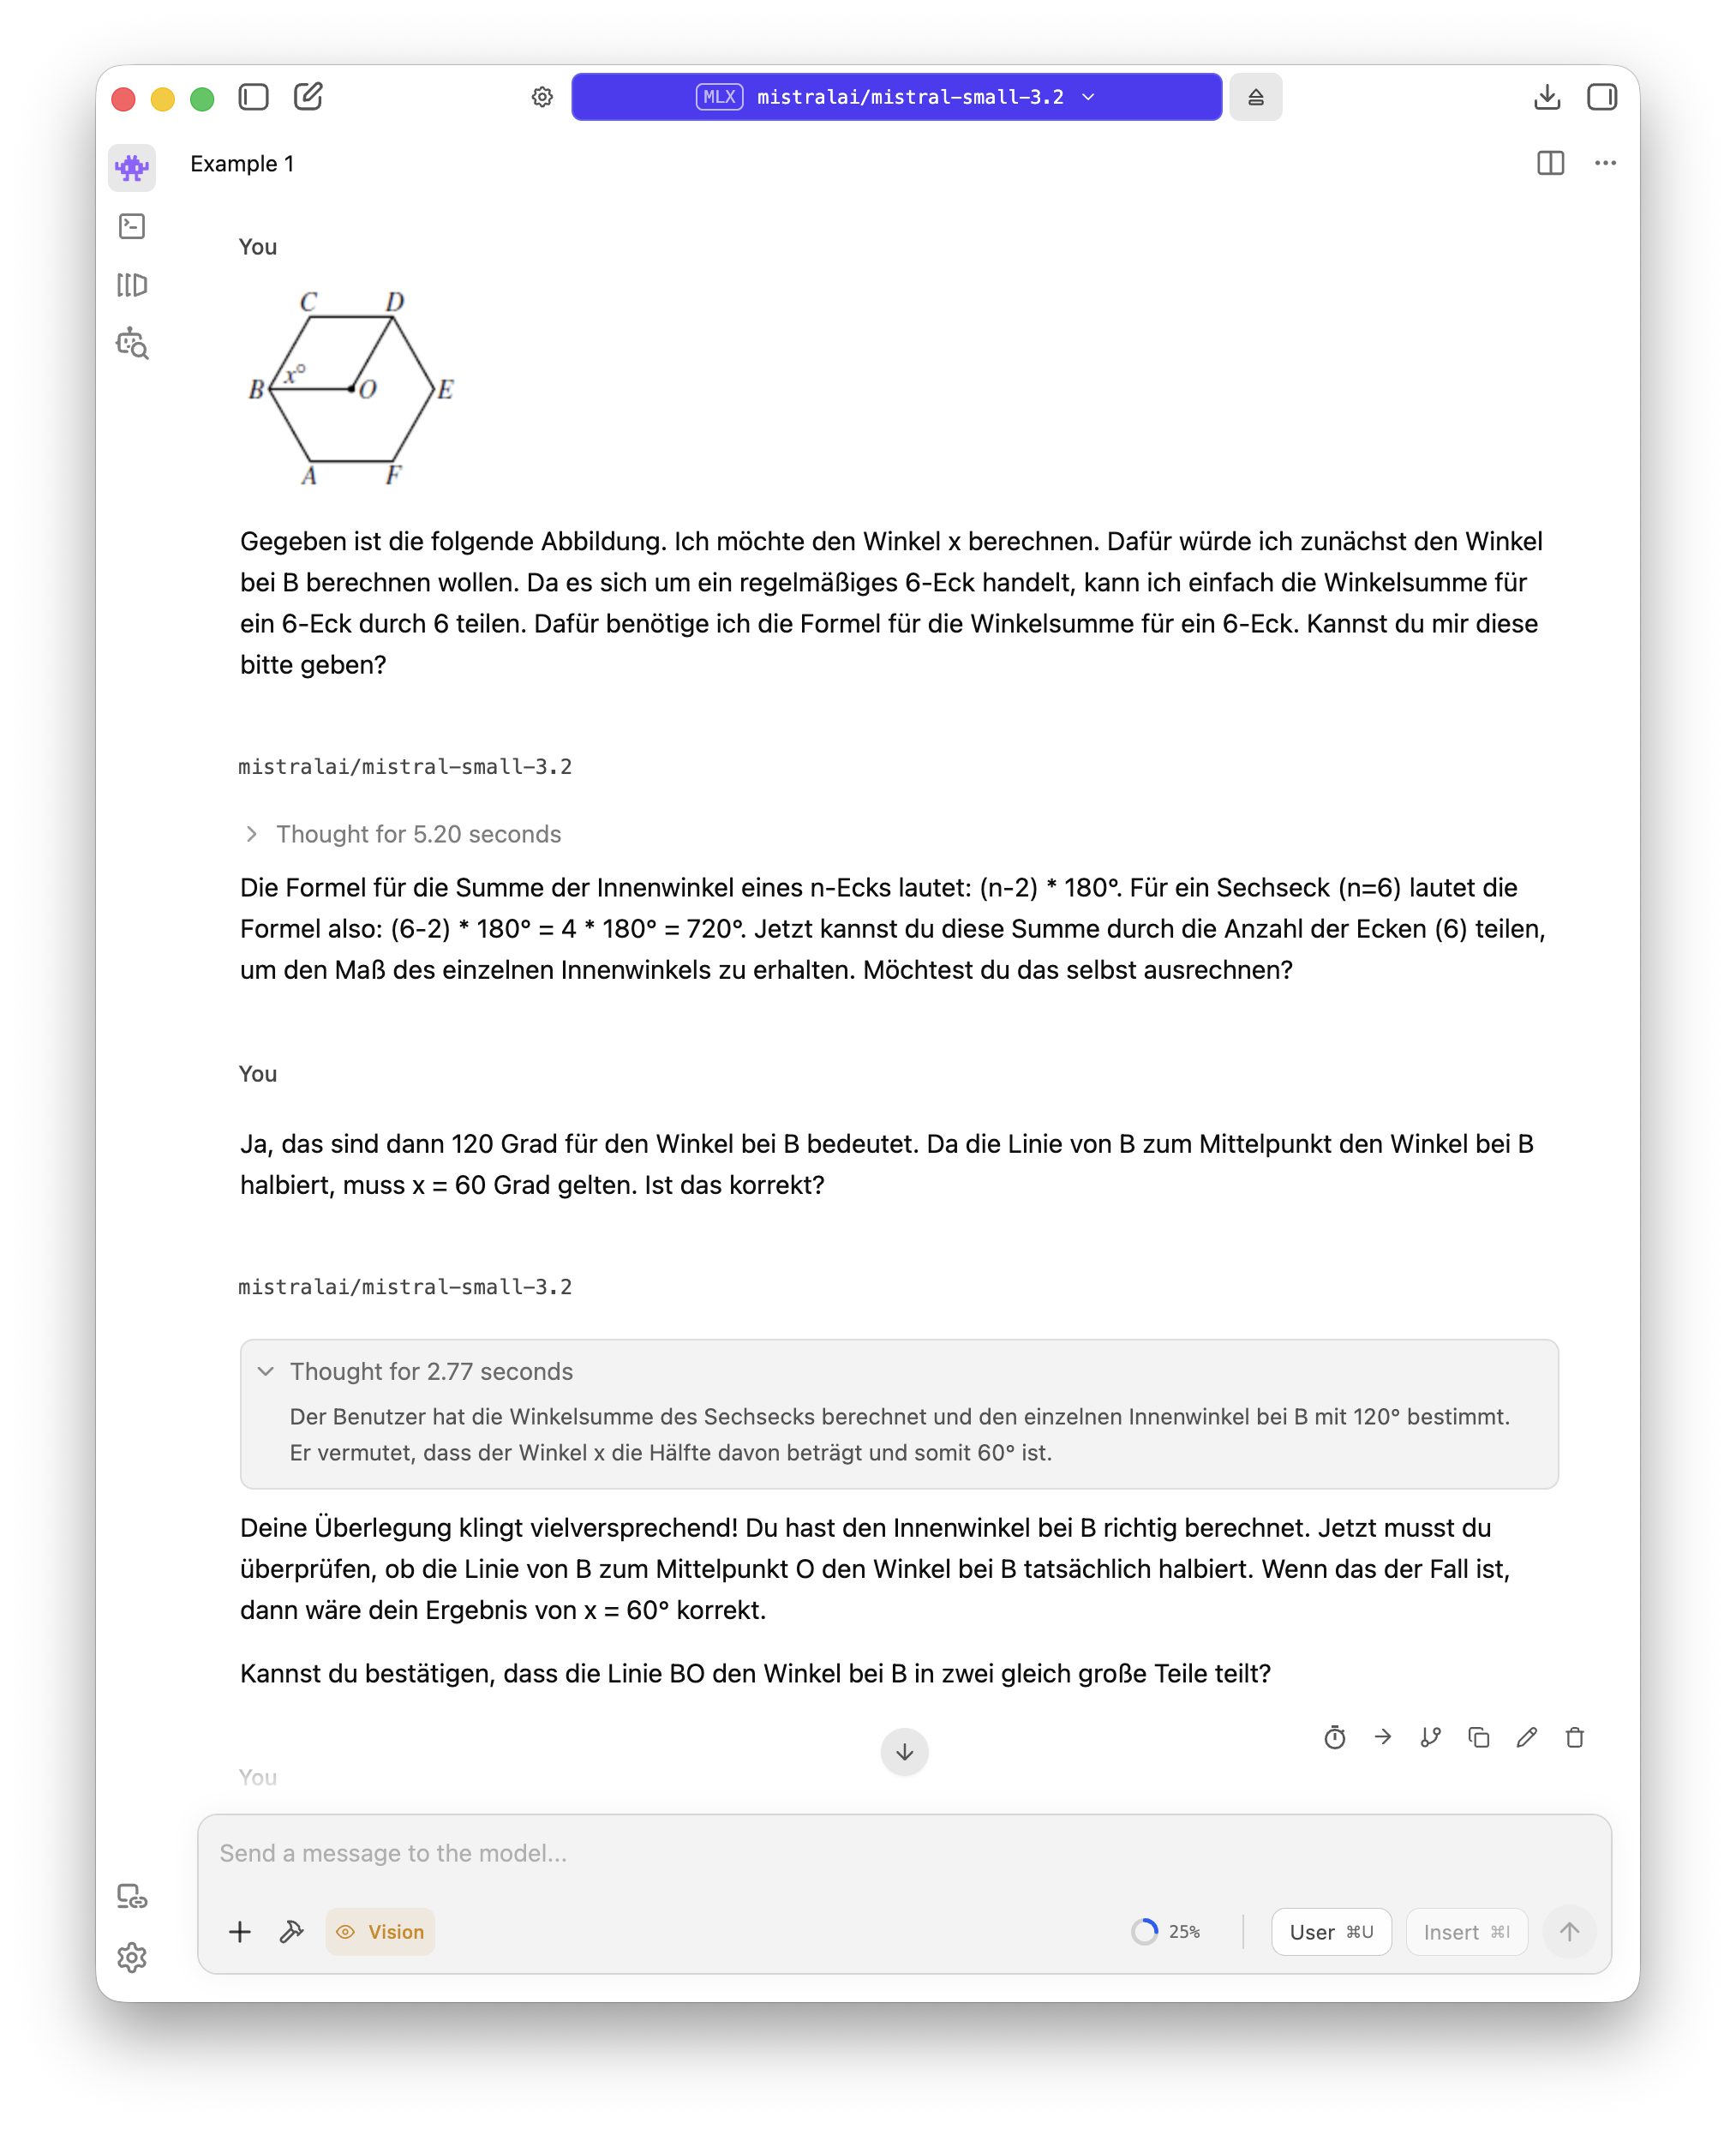
\includegraphics[width=\textwidth]{images/fig-chatbot-explanation.png}
        \caption{Chatbot with explanations}
        \label{fig:chatbot_E}
    \end{subfigure}
    \hfill
    \begin{subfigure}{0.49\textwidth}
        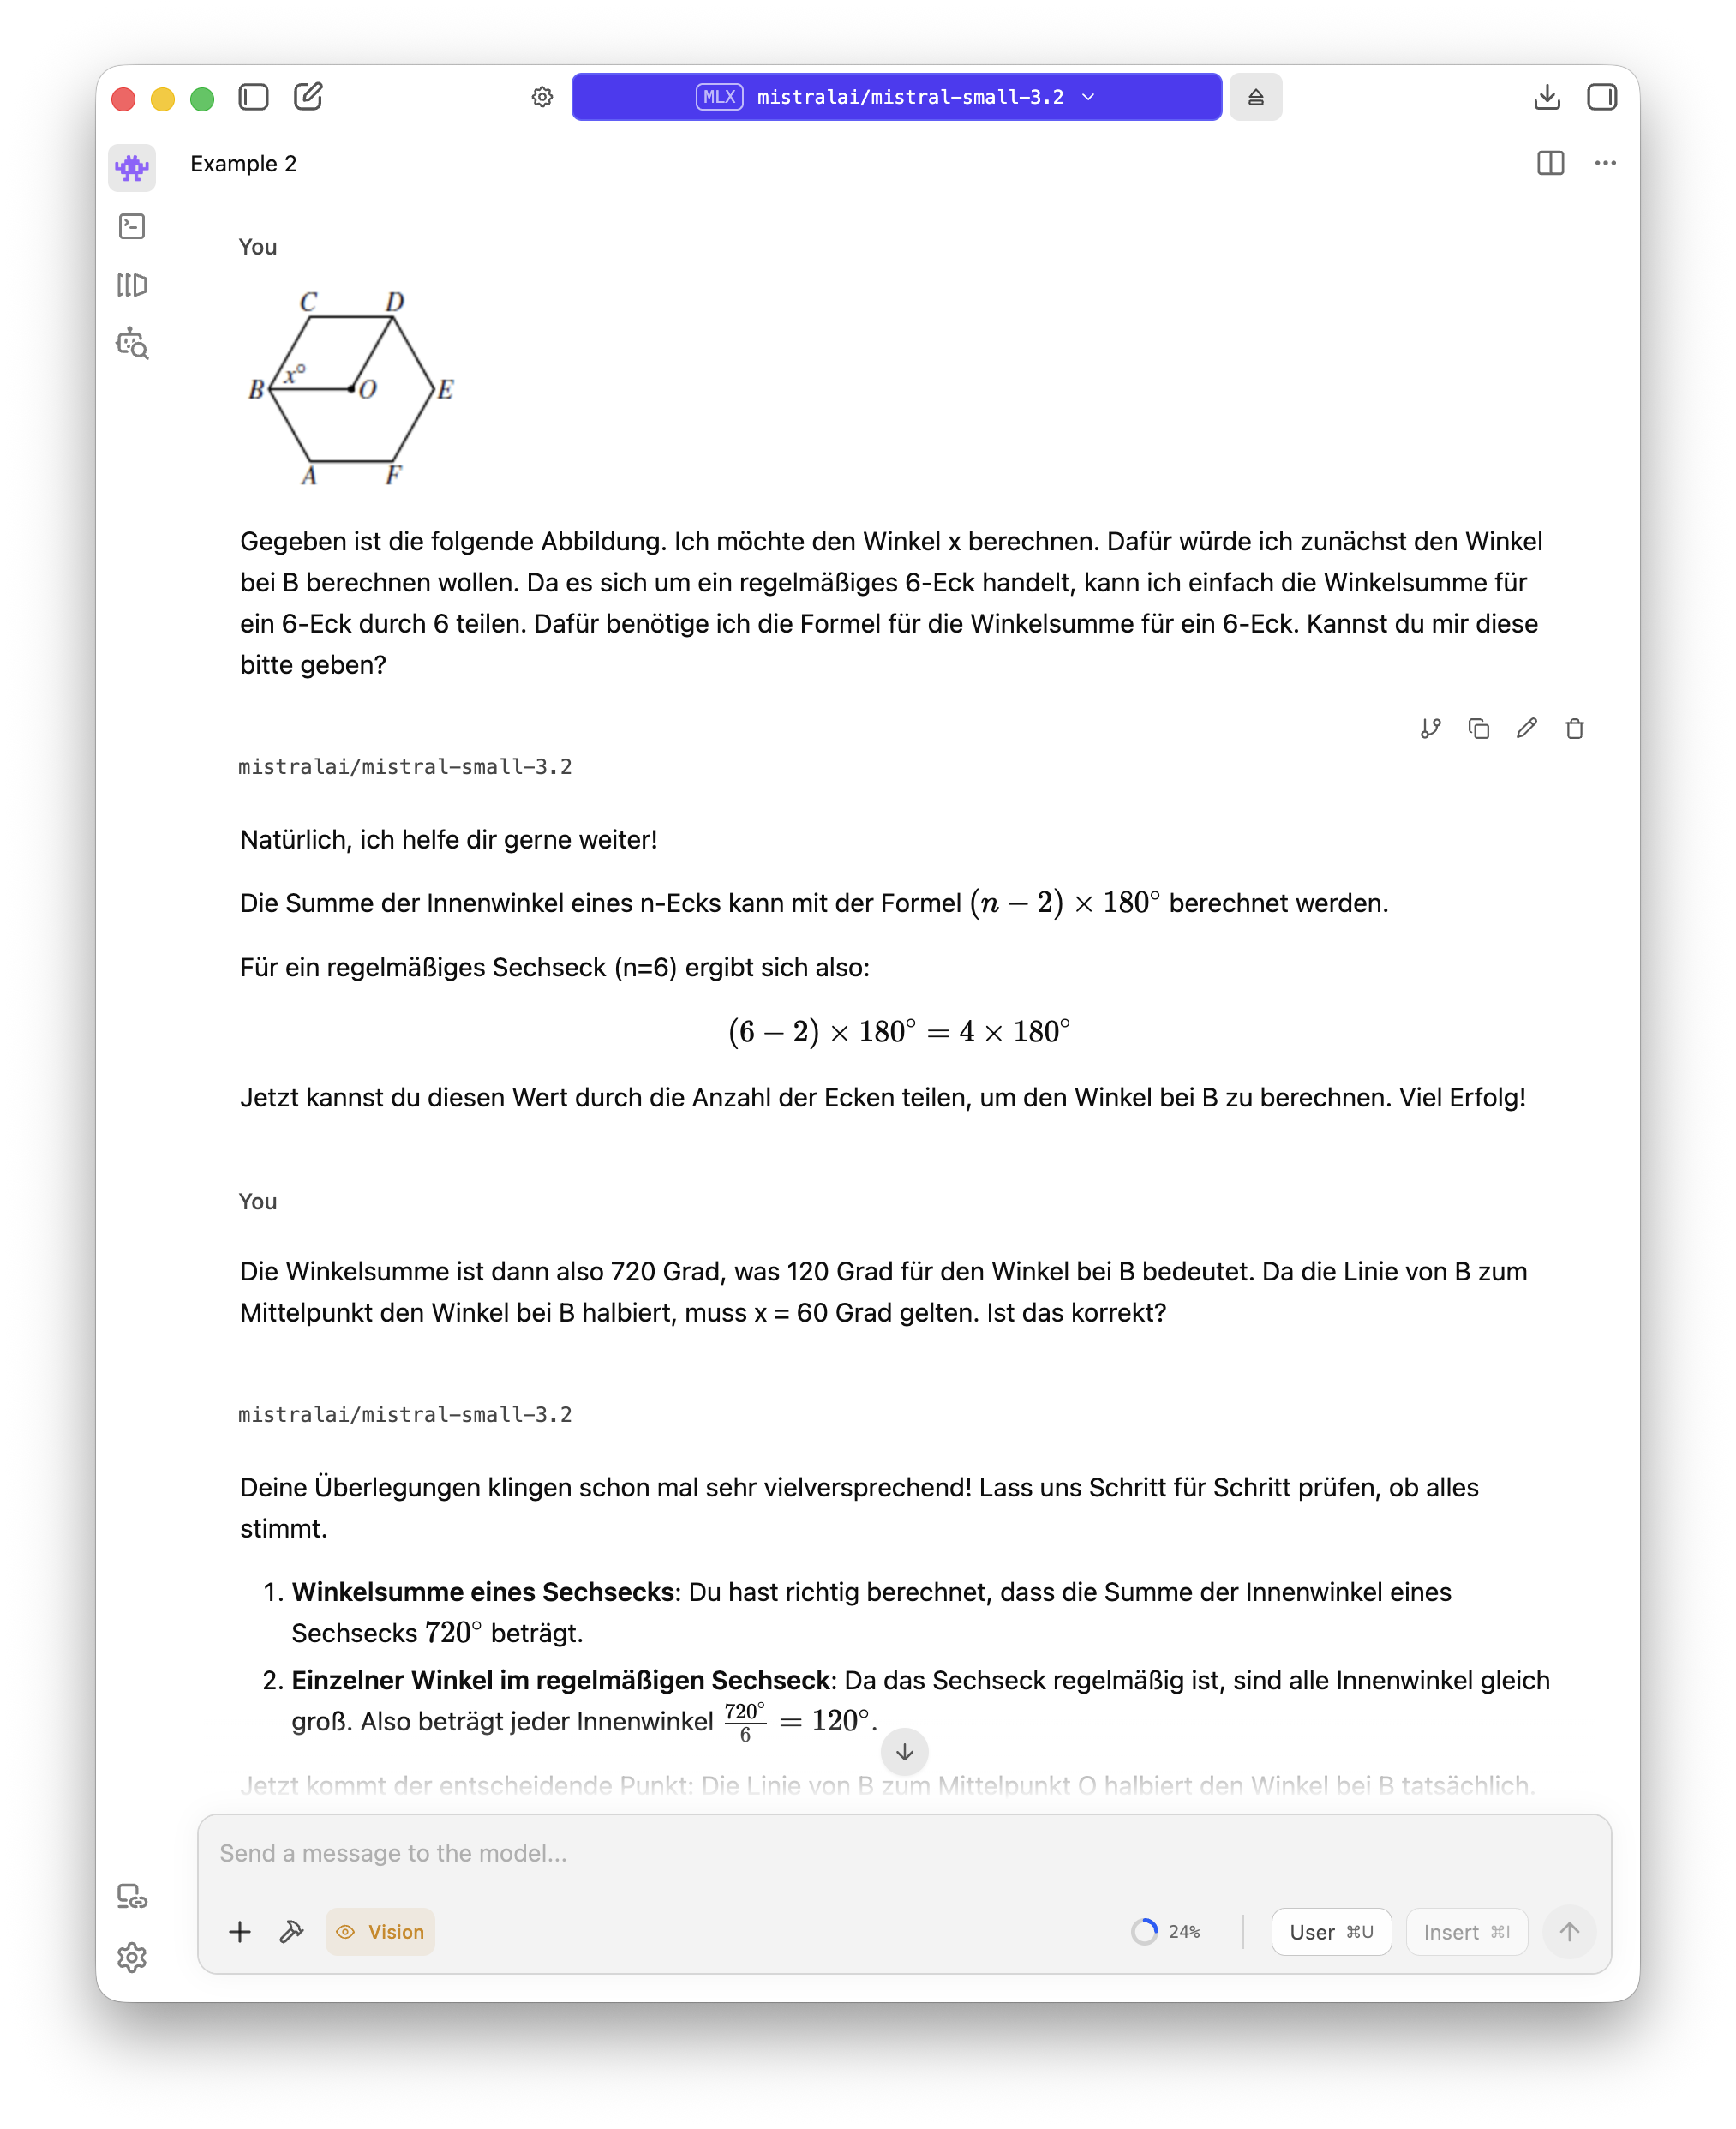
\includegraphics[width=\textwidth]{images/fig-chatbot-control.png}
        \caption{Chatbot without explanations}
        \label{fig:chatbot_C}
    \end{subfigure}
    \caption[Screenshots of chatbot variants]{Screenshots of the introductory task demonstration for both chatbots. The chatbot for group (E) shows the examples of the collapsed and expanded explanations, while the chatbot for group (B) does not show any explanations.}
    \label{fig:chatbots}
\end{figure}
